\documentclass[10pt]{article}

\usepackage{polski}
\usepackage{graphicx}
\usepackage{hyperref}
\graphicspath{{images/}}

\usepackage{geometry}
\newgeometry{tmargin=4cm, bmargin=4cm, lmargin=3.2cm, rmargin=3.2cm}

\usepackage{fancyhdr}
\usepackage{ulem}
\usepackage{float}
\pagestyle{fancy}



\begin{document}

\begin{titlepage}


\begin{center}

  \LARGE \textsc{Politechnika Wrocławska}\\
  \vspace*{0.2cm}
  \Large \textsc{Wydział Informatyki i Telekomunikacji}\\
  \vspace*{0.4cm}
  \centering
\includegraphics[width=0.2\textwidth]{WITlogo.png}\\
  \vspace*{0.2cm}
  \vspace*{2cm}

  \centerline{\rule{\textwidth}{1.2pt}}
  \vspace{0.4cm}
  \Huge\textbf{Metody i Systemy Decyzyjne}
  \centerline{\rule{\textwidth}{1.2pt}}
  \vspace{1cm}
  \LARGE Sprawozdanie z laboratorium\\
  \vspace{3.5cm}
  \textsc{Autor}\\
  \vspace{0.2cm}
  \textbf{Kacper Wójcicki}\\
  \vspace{0.1cm}
  \Large nr albumu: \textbf{260388}\\
  \vspace{0.1cm}
  kierunek: \textbf{Informatyka Stosowana}

  \vspace*{\fill}
  \Large \textit{\today}

 \end{center}


\end{titlepage}


\begin{abstract}
Celem pracy jest zbadanie wpływu alkoholu na takie czynniki życiowe jak szczęście, długość życia i PKB per capita.
Dane zostały pobrane ze strony \url{https://www.wikipedia.org/}.
Analizę przeprowadzono za pomocą regresjii liniwej oraz regresji wielomianowej.
W rezultacie udało się stwierdzić, że istnieje pewna zależność między alkoholem, a wyżej wymienionymi czynnikami życiowymi.
\end{abstract}

\section{Wstęp -- sformułowanie problemu}
\label{sec:wstep}

\textit{Na wstępie warto zaznaczyć, że nasz raport jest jedynie suchą analizą wybiorczych, uśrednionych danych i \textbf{nie powinien być brany pod uwagę jako powód do zwiększenia ilości spożywanego alkoholu}, gdyż jak jest to powszechnie wiadome alkohol szkodzi naszemu zdrowiu.}

Przchodząć do naszego tematu, aby pokazać badane zależności, pobraliśmy dane o średniej liczbie litrów alkoholu wypitych przez ludzi oraz dane takie jak:
\begin{enumerate}
    \item współczynnik szczęścia
    \item średnia długość życia
    \item PKB per capita
\end{enumerate}

\section{Opis rozwiązania}

Dane o wyżej wymionych czynnikach zostały pobrane z ogólnodostępnego źródła jakim jest wikipedia, a dokładnie ze stron podanych poniżej:
\begin{itemize}
    \item \url{https://en.wikipedia.org/wiki/List_of_countries_by_alcohol_consumption_per_capita}
    \item \url{https://en.wikipedia.org/wiki/World_Happiness_Report}
    \item \url{https://en.wikipedia.org/wiki/List_of_countries_by_life_expectancy}
    \item \url{https://en.wikipedia.org/wiki/List_of_countries_by_GDP_(nominal)_per_capita}
\end{itemize}
Z tabel wzięte zostały potrzebne kolumny oraz umieszczone w ramkach danych biblioteki \texttt{Pandas}.
Dla każdego z czynników (współczynnik szczęścia, średnia długość życia oraz PKB per capita) zostały stworzone osobne zależności od alkoholu wypitego na osobę poprzez użycie regresji liniowej oraz regresji wielomianowej 4 stopnia, dzięki której mamy dokładniejsze spojrzenie na zależność.
Użyłem do tego funkcji \texttt{polyfit()} z bilbioteki \texttt{numpy}, która używa metody najmniejszych kwadratów do wyznaczenia tych regresjii.
\pagebreak
\section{Rezultaty obliczeń}

\subsection{Plan badań}
Dla ułatwienia obliczeń do danych wziąłem średnie wartości w 144 krajach.
Zatem jeden "rekord" danych jest dla jednego kraju.
Przykładowe przetworzone dane pokazano w tabeli poniżej:

\begin{table}[H]
    \begin{tabular}{|l|l|l|l|l|l|}
    \hline
    \textbf{Kraj}  & \textbf{Alkohol per capita} & \textbf{Współczynnik Szczęścia} & \textbf{Średnia długość życia} & \textbf{PKB per capita} \\ \hline
    Finlandia & 10.7 & 7.809 & 82.13 & 48773.0   \\ \hline
    Mołdawia & 15.2 & 5.608 & 72.01 & 4551.0   \\ \hline
    Peru & 6.3 & 5.797 & 76.95 & 6127.0   \\ \hline
    Wietnam & 8.3 & 5.353 & 75.49 & 2786.0   \\ \hline
    Zimbabwe & 4.8 & 3.299 & 61.74 & 1128.0  \\ \hline
    Serbia & 11.1 & 5.778 & 74.23 & 7721.0   \\ \hline
    \end{tabular}
    \caption{Dane dla przykładowych krajów}
\end{table}

\subsection{Wyniki obliczeń}
\subsubsection{Zależność współczynnika szczęścia od alkoholu}
Oto jak zależność przedstawia się na wykresach:
\begin{figure}[H]
    \begin{center}
        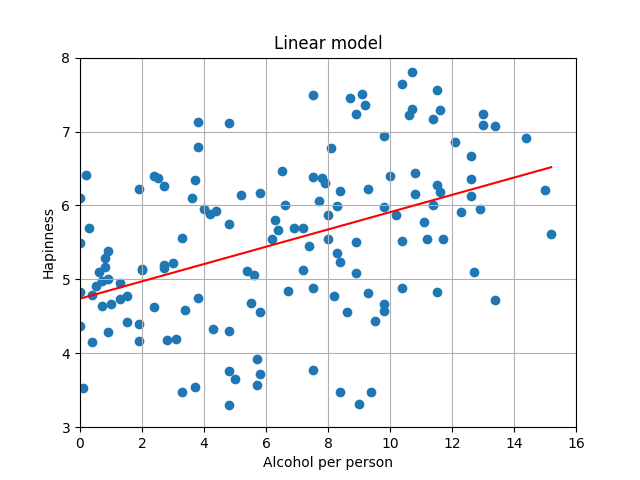
\includegraphics[width=0.8\linewidth]{plots/happiness_dependence_linear.png}
        \caption{Zależność liniowa współczynnika szczęścia od wypitego alkoholu}
    \end{center}
\end{figure}

\begin{figure}[H]
    \begin{center}
        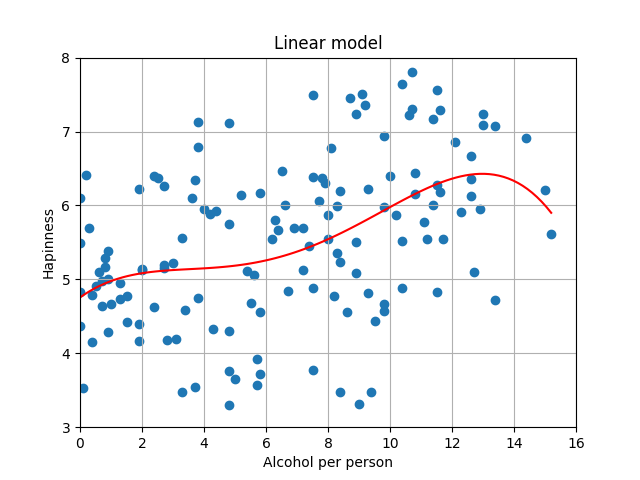
\includegraphics[width=0.8\linewidth]{plots/happiness_dependence_poly.png}
        \caption{Zależność wielomianowa współczynnika szczęścia od wypitego alkoholu}
    \end{center}
\end{figure}

Z wykresu regresji liniowej można spostrzec, że trend jest taki, że im więcej alkoholu rocznie pijemy tym szczęśliwsi jesteśmy, ale na dokładniejszym wykresie regresji wielomianowej widać, że można przesadzić z alkoholem, co prowadzi do obniżenia naszego poziomu szczęścia.

\pagebreak
\subsubsection{Zależność średniej długości życia od alkoholu}
Warto tutaj przypomnieć, że operujemy tylko na suchych danych i odkładamy naszą wiedzę medyczną na bok, gdyż wiadomym jest że alkohol szkodzi naszemu zdrowiu, a nie wydłuża nasze życie.
Jednak same dane na wykresach prezentują się następująco:

\begin{figure}[H]
    \begin{center}
        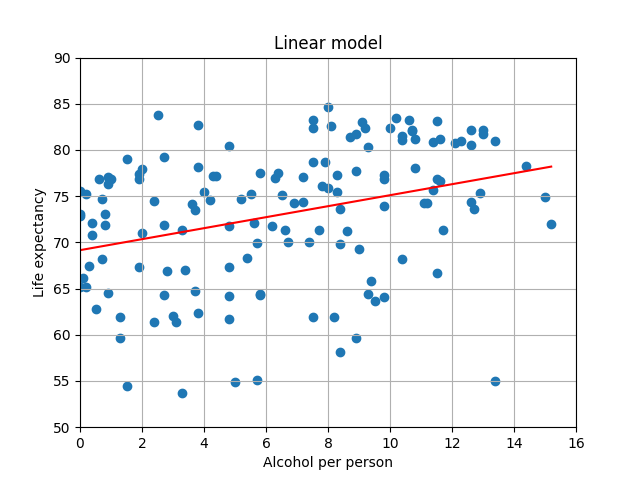
\includegraphics[width=0.8\linewidth]{plots/life_expectancy_dependence_linear.png}
        \caption{Zależność liniowa średniej długości życia od wypitego alkoholu}
    \end{center}
\end{figure}

\begin{figure}[H]
    \begin{center}
        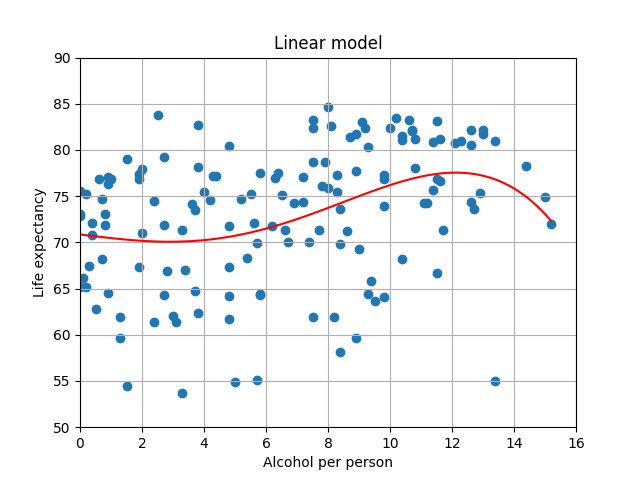
\includegraphics[width=0.8\linewidth]{plots/life_expectancy_dependence_poly.png}
        \caption{Zależność wielomianowa średniej długości życia od wypitego alkoholu}
    \end{center}
\end{figure}

Co ciekawe na wykresach można zaobserwować praktycznie taką samą zależność jak przy współczynniku szczęścia.

\pagebreak
\subsubsection{Zależność PKB per capita od alkoholu}
Dane na wykresach prezentują się następująco:

\begin{figure}[H]
    \begin{center}
        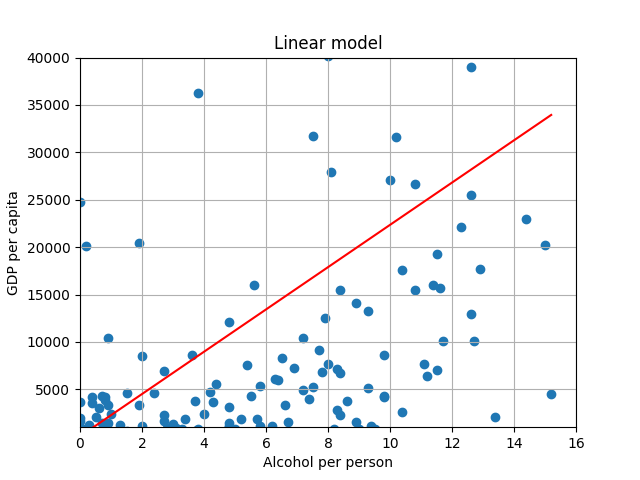
\includegraphics[width=0.8\linewidth]{plots/GDP_dependence_linear.png}
        \caption{Zależność liniowa PKB per capita od wypitego alkoholu}
    \end{center}
\end{figure}

\begin{figure}[H]
    \begin{center}
        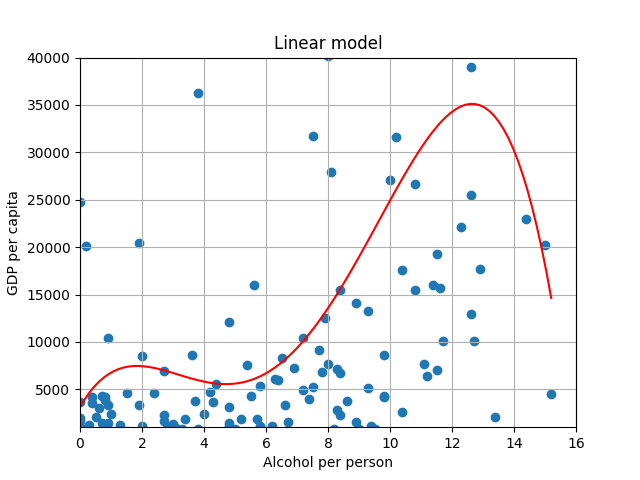
\includegraphics[width=0.8\linewidth]{plots/GDP_dependence_poly.png}
        \caption{Zależność wielomianowa PKB per capita od wypitego alkoholu}
    \end{center}
\end{figure}

Tutaj zależność prezentuje się trochę inaczej.
Z wykresu regresji liniowej możnaby przypuszczać, że wartości są do siebie wprostproporcjonalne, czyli im więcej rocznie wypijemy litrów alkoholu tym nasze PKB będzie większe.
Jednak na wykresie regresji wielomianowej widać, że nie do końca tak jest.
Obserwujemy duży przyrost po lokalnym minimum przy 6 litrach wypitych rocznie, aż do maksimum w ok. 12,5 litrach, po czym duży spadek.

\section{Wnioski}
Pokazane wyżej zależności wskazują na fakt, że ogólnie alkohol daje nam szczęście, wydłuża życie oraz pomaga nam rozwijać się finansowo - z zastrzeżeniem, że możemy przesadzić z ilością wypitego alkoholu co może skutkowac nagłą obniżką tych wartości.
Myślę że każdy po przeczytaniu powyższego zdania miał co do niego mieszane myśli, bo przecież wszyscy wiemy, że alkohol szkodzi zdrowiu.
Pokazuje to jak trudno jest znaleźć zależności w prawdziwym świecie, w tym także co od czego zależy oraz jak szeroki kontekst potrzbujemy do określenia zależności.
Suche dane często nie wystarczają.
Znając powyższe warto byłoby przemyśleć odwrotną zależność np. ilość wypitego alkoholu od PKB.

\pagebreak
\appendix
\section{Dodatek}
Kody źródłowe umieszczone zostały w repozytorium github:

\noindent \url{https://github.com/Bodzisz/Alcohol-Influence-On-Life-Factors}.


\end{document}
